\section{Dwi Septiani Tsaniyah(1174003)}
\subsection{Intalasi Map Proxy}
\begin{enumerate}
    \item Gunakan perintah pip install map proxy pada cmd
    \hfill\break
    \begin{figure}[H]
		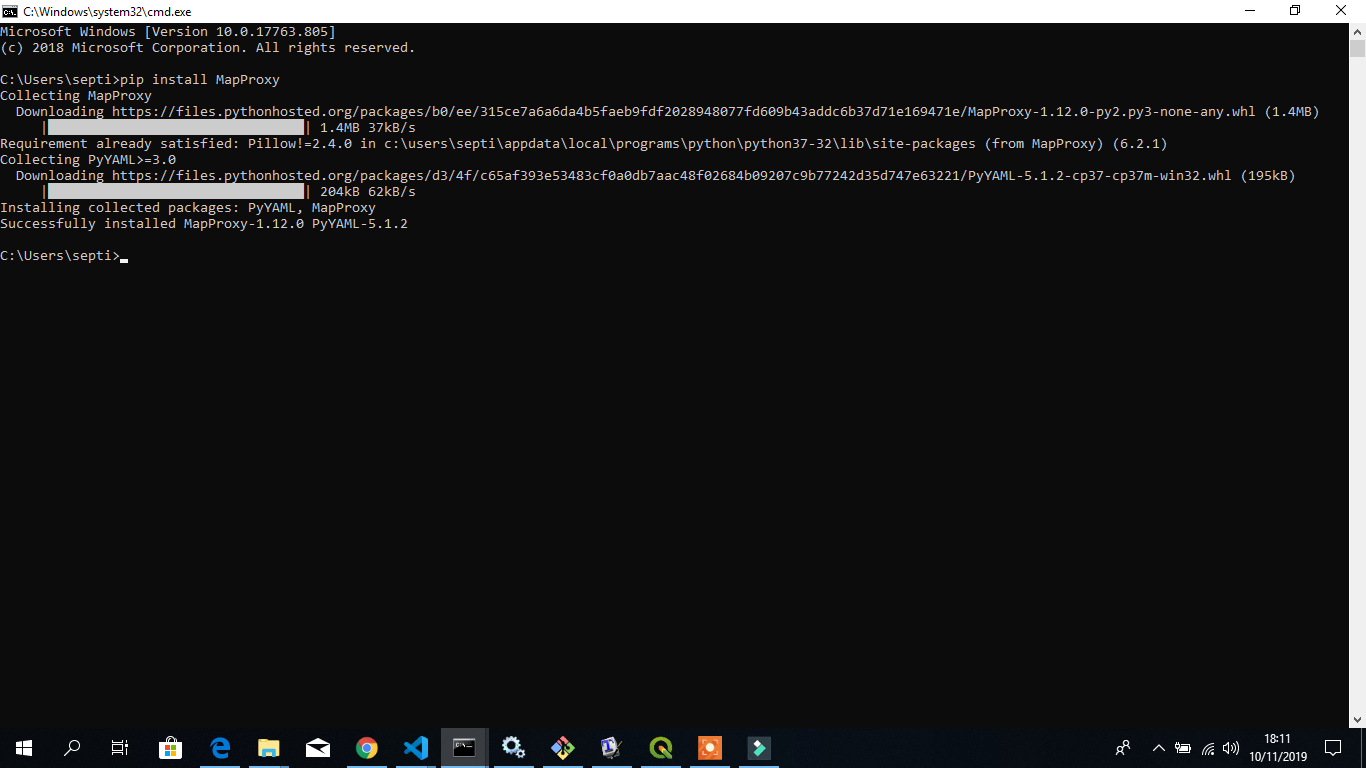
\includegraphics[width=4cm]{figures/1174003/5/1.png}
		\centering
		\caption{Perintah untuk menginstal map proxy}
    \end{figure}
\end{enumerate}
\subsection{Konfigurasi}
\begin{enumerate}
    \item Download filenya terlebih dahulu pada \href{https://github.com/awangga/gede}{Github Pa Rolly yang mengemaskan}
    \hfill\break
    \begin{figure}[H]
		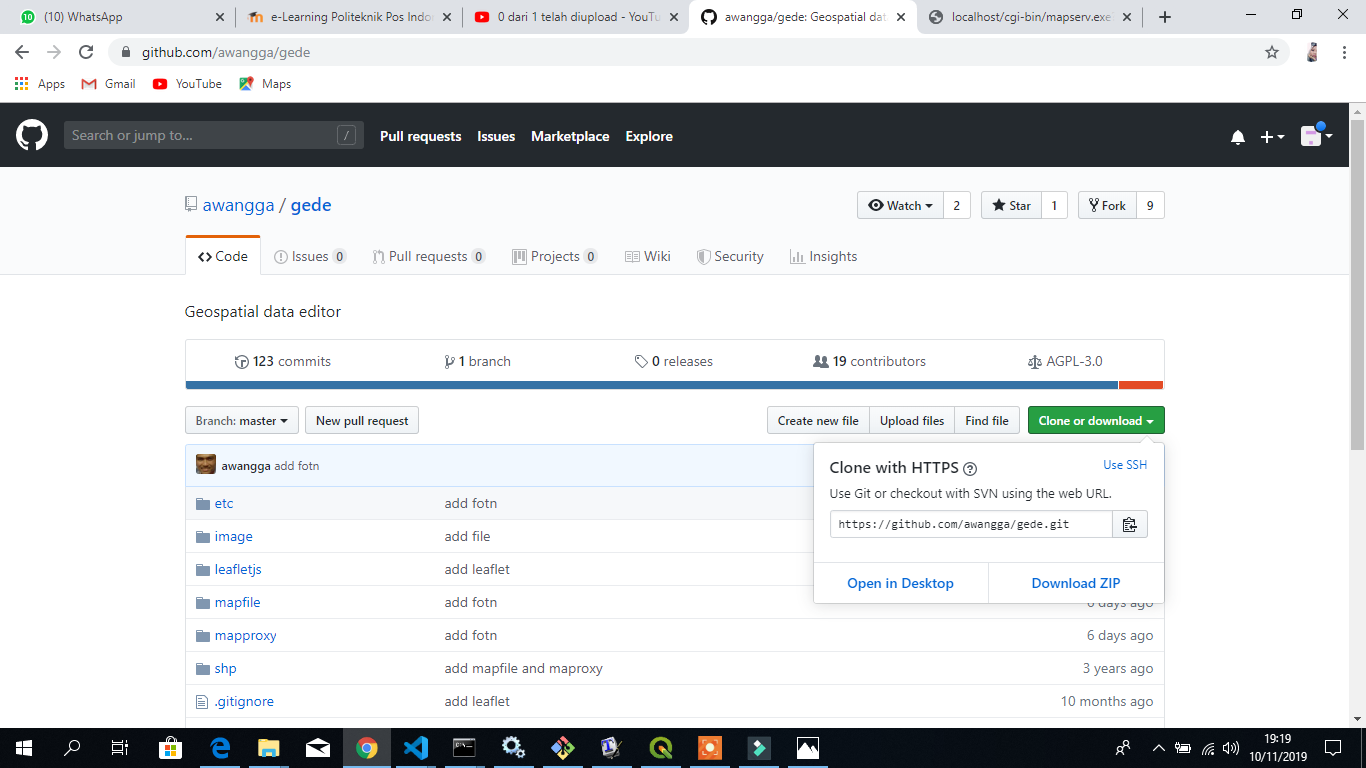
\includegraphics[width=4cm]{figures/1174003/5/2.png}
		\centering
		\caption{Download file untuk melakukan konfigurasi}
    \end{figure}
    \item Setelah didownload kemdian lakukan extrack
    \hfill\break
    \begin{figure}[H]
		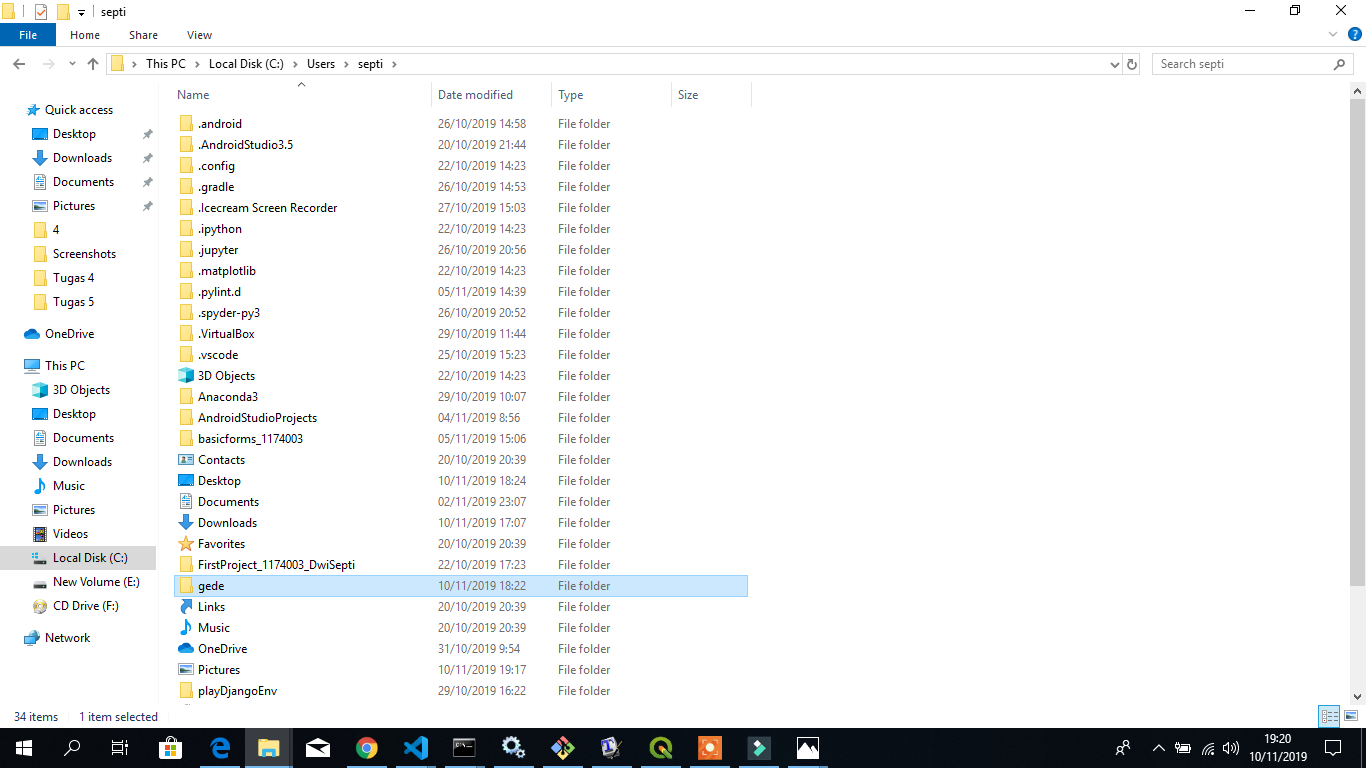
\includegraphics[width=4cm]{figures/1174003/5/3.png}
		\centering
		\caption{Extrack}
    \end{figure}
    \item Buka file agm.yaml, dan ubah binarynya serta working dirnya
    \hfill\break
    \begin{figure}[H]
		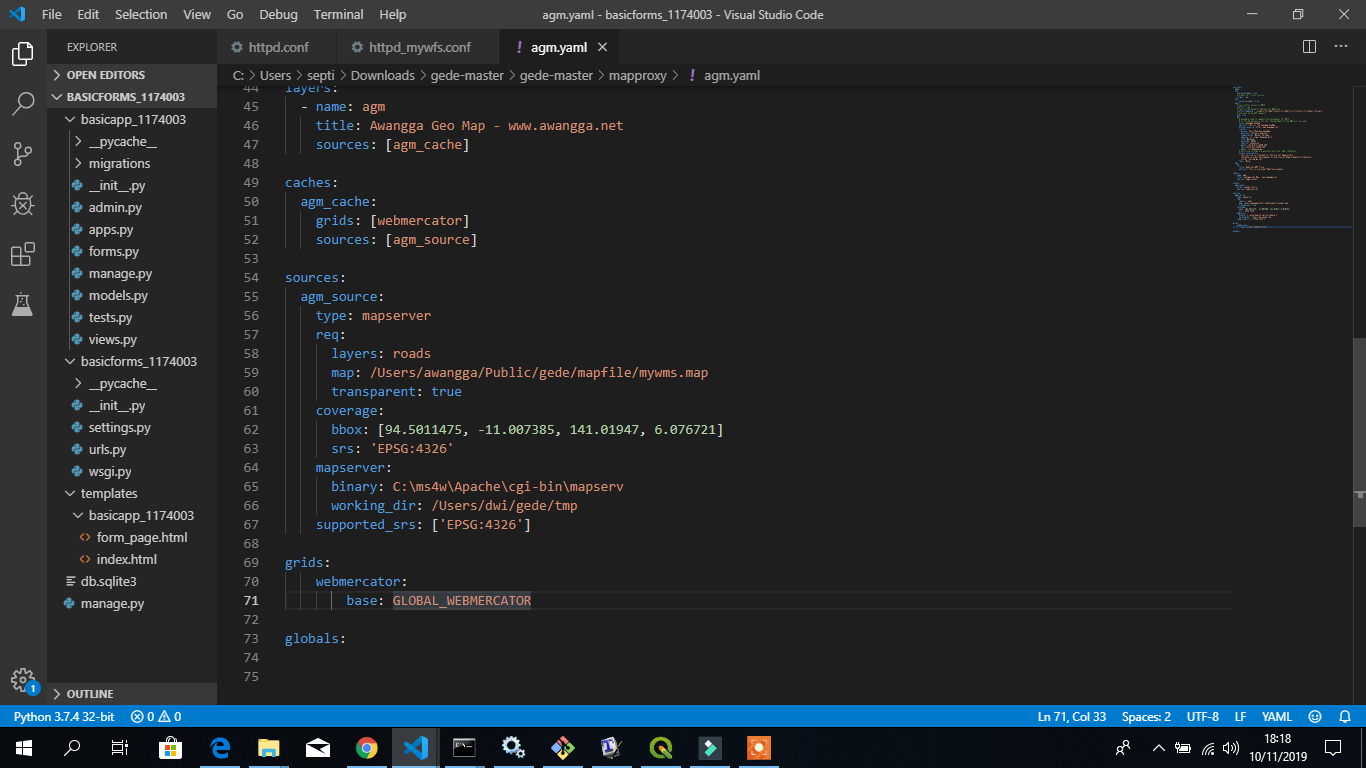
\includegraphics[width=4cm]{figures/1174003/5/4.png}
		\centering
		\caption{Ubah binary dan working dir}
    \end{figure}
    untuk binarynya sesuai dengan tempat map servernya
\end{enumerate}
\subsection{Pengujian}
\begin{enumerate}
    \item Untuk melakukan pengujian bisa dengan menggunakan perintah mapproxy-util serve-develop mapproxy.yaml -b 0.0.0.0:8181
    \hfill\break
    \begin{figure}[H]
		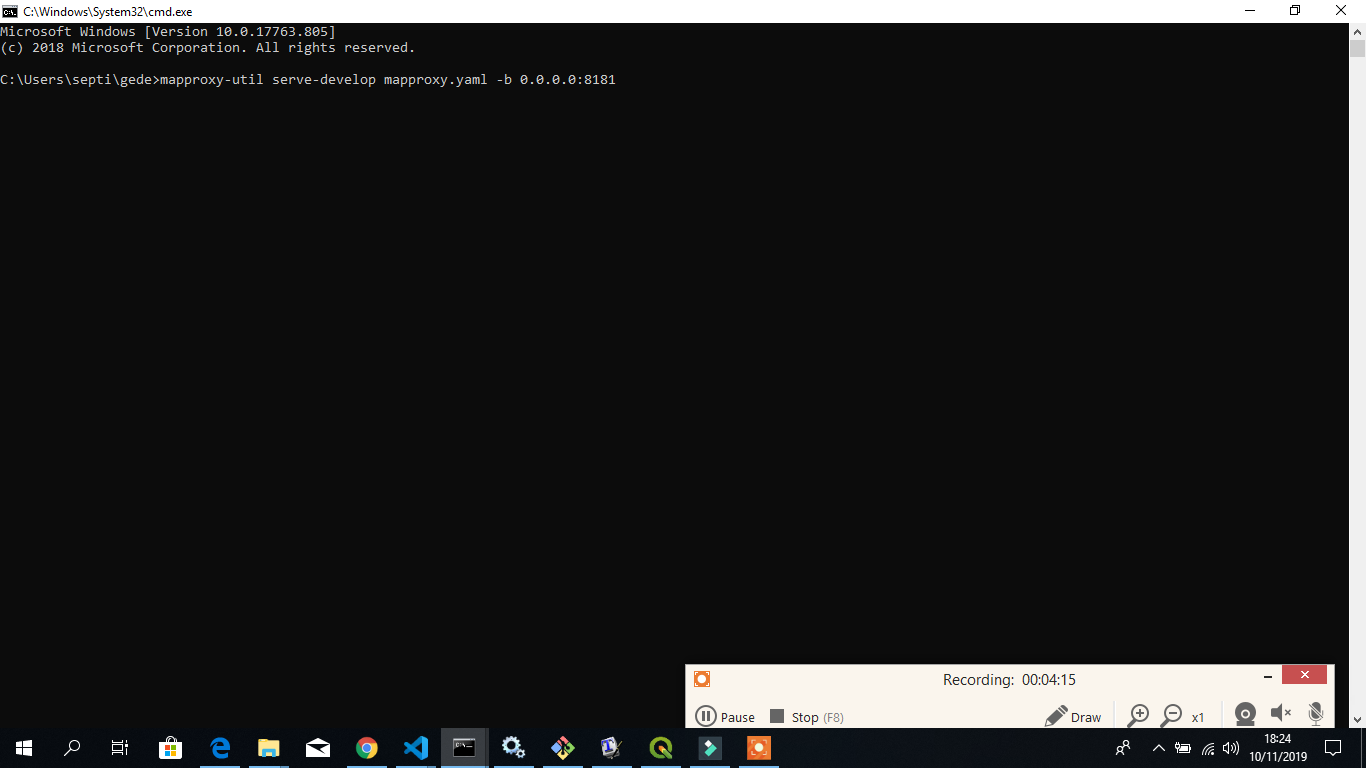
\includegraphics[width=4cm]{figures/1174003/5/5.png}
		\centering
		\caption{Perintah untuk menjalankan mapproxy}
    \end{figure}
\end{enumerate}
\subsection{Link Youtube}
\href{https://youtu.be/zAVZDnuP8K8}{Klik Disini}